\documentclass[../thesis.tex]{subfiles}
\begin{document}
\chapter{Transient and Steady-State Dynamics}

This section is referencing my paper.\cite{Hershey2016,Hershey2017}
\section{Motivation}
\section{Theory}
\subsection{Previous Efficiency Roll-Off Models}
\section{Exciton Dynamics}
\begin{equation}
\frac{dn_{ex}}{dt} = - \frac{n_{ex}}{\tau}-\frac{1}{2}k_{TT}n_{ex}^2-k_{TP}n_{pol}n_{ex}+G_{ex}
\label{eqn:exciton_rate}
\end{equation}

\begin{equation}
G_{ex}=\frac{k_F}{4}n_{pol}^2
\label{eqn:exciton_formation}
\end{equation}


\section{Polaron Dynamics}

\begin{equation}
\frac{dn_{pol}}{dt}=\frac{-k_F}{2}n_{pol}^2-\frac{n_{pol}}{\tau_l}+G_{pol}
\label{eqn:polaron_rate}
\end{equation}

\section{Exciton Quenching in Photoluminescence}

\begin{equation}
V=\left[ \frac{J}{e\mu N_C}d^{2l+}\left( \frac{eN_0k_BT_t}{\epsilon} \right)^l \right]^{\frac{1}{l+1}}=CJ^{\frac{1}{l+1}}
\label{eqn:ktpVoltage}
\end{equation}

\begin{equation}
n_{pol}=eN_c\left(\frac{\epsilon V}{ed^2N_0kT_t}\right)^l
\label{eqn:kptDensity}
\end{equation}

\begin{equation}
\frac{L(n_{pol}}{L_0}=\frac{1}{1+\tau k_{TP}n_{pol}}
\label{eqn:ktpFit}
\end{equation}




\begin{wrapfigure}{r}{0.5\textwidth}
\centering
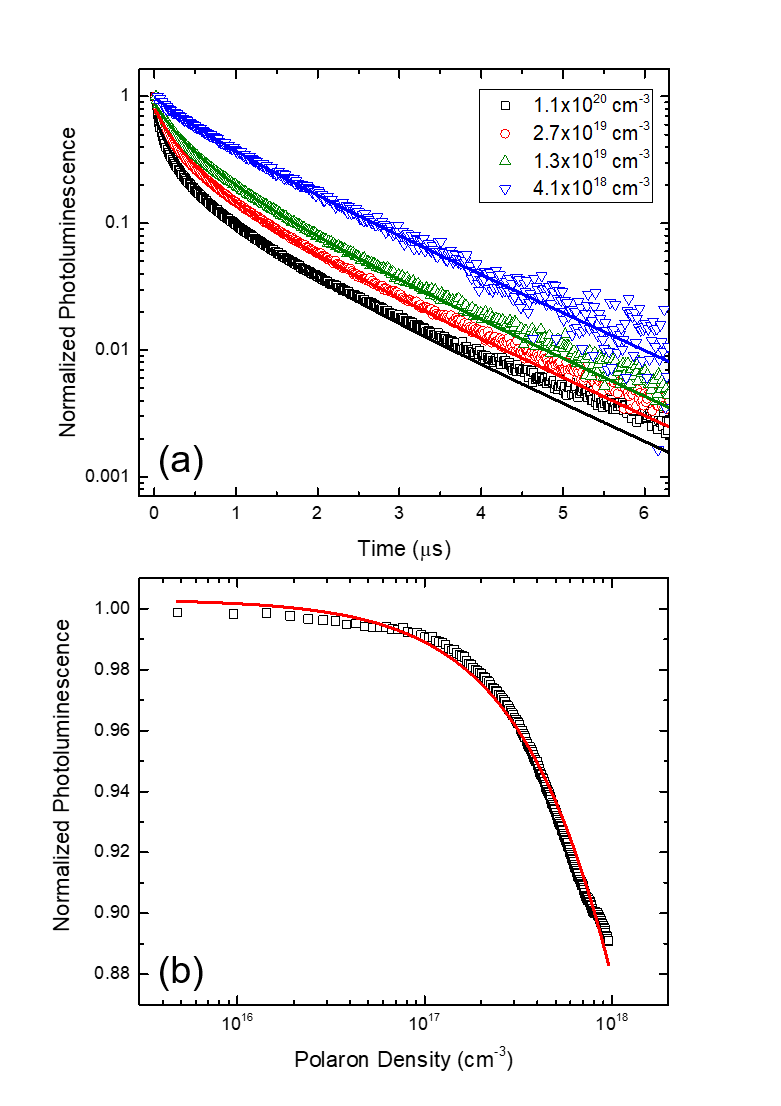
\includegraphics[width=0.48\textwidth]{unified/PL_fitting}
\caption{(a) Transient photoluminescence (PL) decays for several initial exciton densities with fits shown as solid lines using Eqn. \ref{eqn:exciton_formation}.  Fit parameters are discussed in SECTION.  Exciton densities are calculated using measured incident power and beam size in combination iwht Beer's Law.  (b) Steady-state PL quenching as a function of polaron density and the resulting fit from Eqn. \ref{eqn:ktpFit} shown as the solid line.}
\label{fig:PL_fitting}
\end{wrapfigure}
\subsection{Transient Electroluminescence}
\subsection{Efficiency Analysis}

\begin{equation}
\eta_{EQE}=\eta_{OC}\eta_{PL}\chi\eta_{EF}
\label{eqn:eqeSimple}
\end{equation}

\begin{equation}
\eta_{EQE}=\frac{\eta_{OC}\eta_{ex}k_r}{G_{pol}/2}
\label{eqn:eqeReform}
\end{equation}

\begin{equation}
\eta_{EF}=\frac{\frac{1}{2}k_Fn_{pol}}{G_{pol}}=\frac{\frac{1}{2}k_Fn_{pol}}{\frac{1}{2}k_Fn_{pol}+\frac{1}{\tau_l}}
\label{eqn:excitonFormation}
\end{equation}

\section{Experimental Details}
\section{Application to Devices}
\subsection{Overview of Approach}
\subsection{Initializing Parameters with Quenching Only Steady-State Model}
\begin{wrapfigure}{r}{0.5\textwidth}
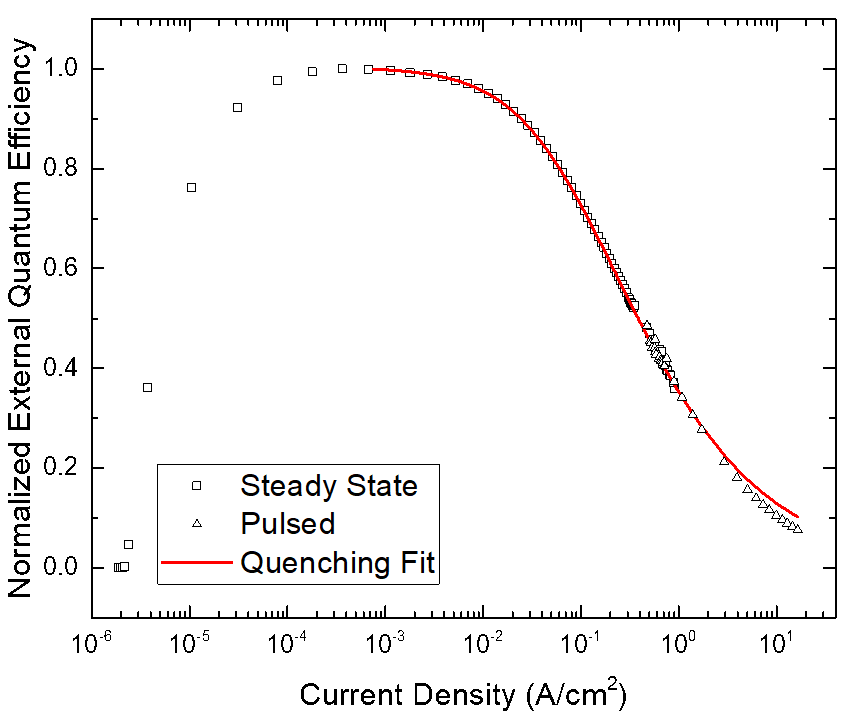
\includegraphics[width=0.48\textwidth]{unified/rollOffFit}
\caption{Normalized experimental $\eta_{EQE}$ as a function of current density.  Solid line is a fit to the data using Eqn. \ref{eqn:exciton_rate} and \ref{eqn:polaron_rate} in the absence of polaron loss.  Pulsed $\eta_{EQE}$ measurements are conducted using low duty cycle pulses to steady-state luminance to reduce Joule heating in device.}
\label{fig:rollOffFit}
\end{wrapfigure}
\subsection{Transient Modeling}
\begin{wrapfigure}{r}{0.5\textwidth}
\centering
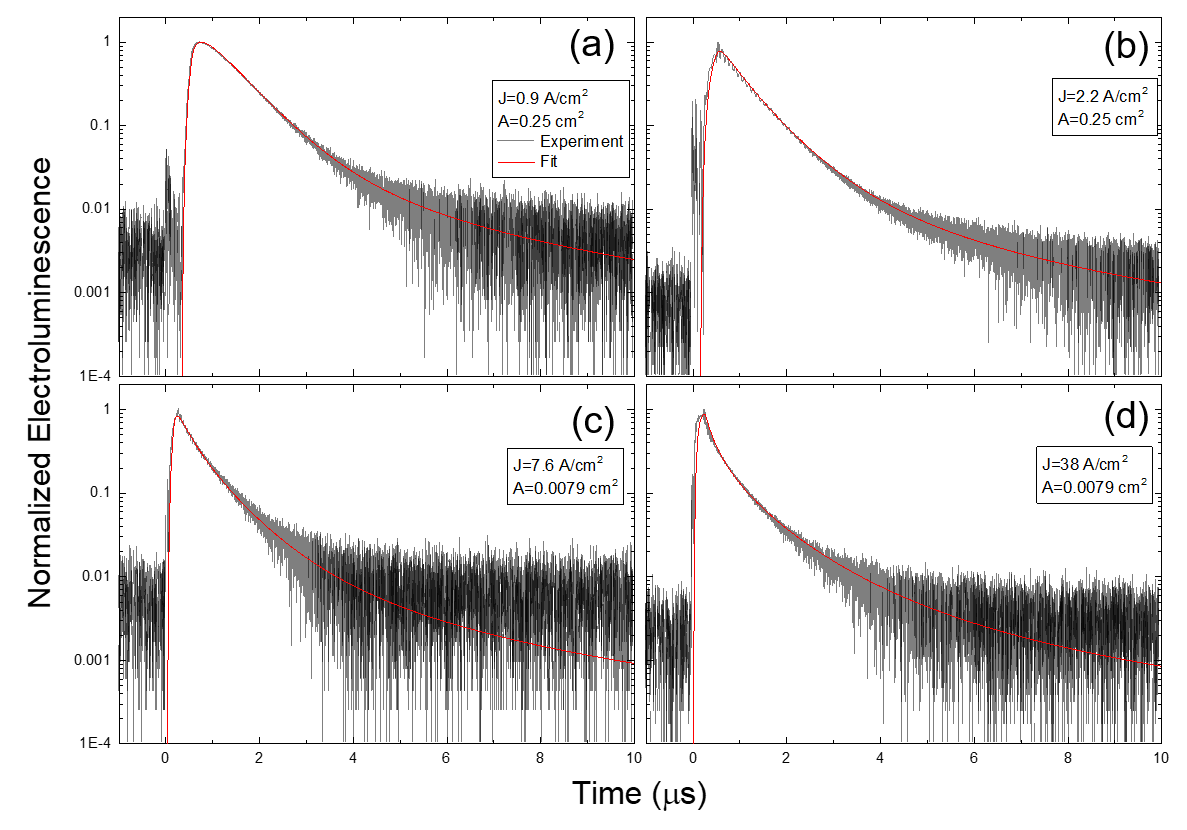
\includegraphics[width=0.48\textwidth]{unified/transientFits}
\caption{Transient electroluminescence (EL) for four different current densities (J) and device areas (A). (a) 0.25 $cm^2$ device at a current density during the pulse of J = 0.9 $A/cm^2$ (b) 0.25 cm2
device at J = 2.2 $A/cm^2$ (c) 0.0079 $cm^2$ device at J = 7.6 $A/cm^2$ (d) 0.0079 $cm^2$ device at J = 38 $A/cm^2$}
\label{fig:transientFits}
\end{wrapfigure}

\begin{table}[h]
\centering
\begin{tabular}{c|c|c}
& Transient EL & Efficiency Roll-off \\
\hline
$\tau$ (s) & $6.9\pm 0.1 \times 10^{-7}$ & $6.1 \times 10^{-7}$ \\
$k_{TT}$ (cm$^3$/s) & $7.1\times 10^{-12}$ &$7.1\times 10^{-12}$ \\
$k_{TP}$ (cm$^3$/s) & $3.3\times 10^{-13}$ &$3.3\times 10^{-13}$ \\
$k_{F}$ (cm$^3$/s) & $7.7\pm3.5\times 10^{-12}$ &$1.6\times 10^{-11}$ \\
\end{tabular}
\caption{Fit parameters extracted from transient and steady-state electroluminescence.  Transient EL fit parameters averaged over all measured current densities.  $\eta_{EQE}$ roll-off parameters averaged over several measured devices.  Triplet-triplet annihilation and triplet-polaron quenching rates are fixed to those obtained from fitting the normalized efficiency roll-off.}
\label{tab:fit_parameters}
\end{table}
% 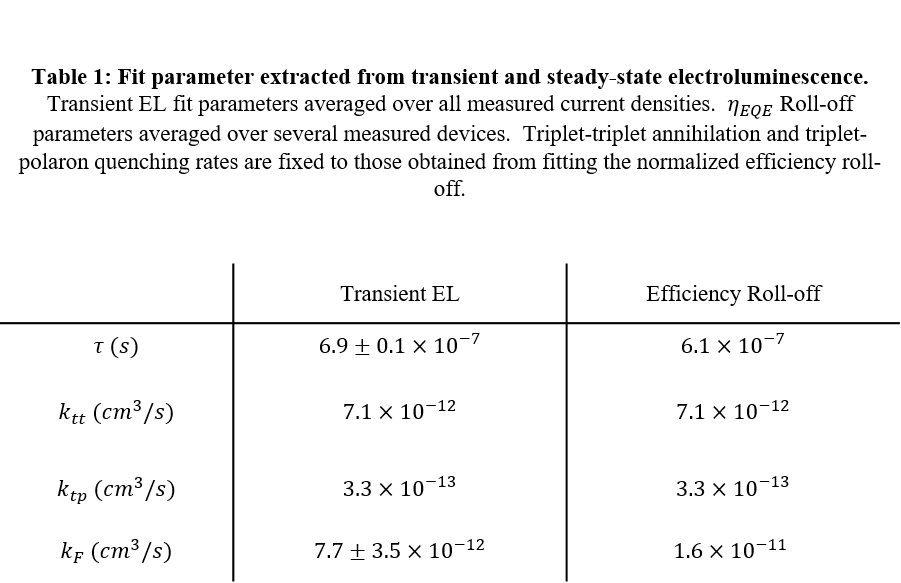
\includegraphics[width=0.48\textwidth]{unified/valueTable}
\subsection{Term Efficiency During Transient}


\begin{wrapfigure}{r}{0.5\textwidth}
\centering
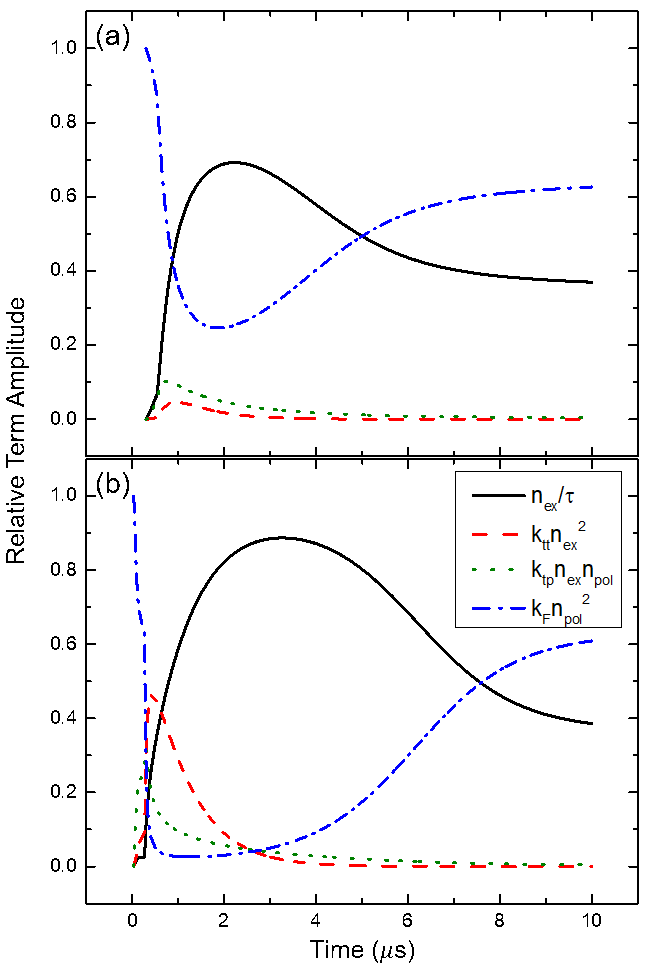
\includegraphics[width=0.48\textwidth]{unified/termEfficiency}
\caption{Term efficiency for each dynamical process influencing the exciton population for (a) 0.25 $cm^2$ device operated at 0.9 $A/cm^2$ for 500 ns and (b) 0.785 $mm^2$ device operated at a current density of 38 $A/cm^2$ for 250 ns. Relative term amplitude is calculated as the magnitude of each term in Eqn. \ref{eqn:exciton_rate} divided by the sum of absolute values of each term.}
\label{fig:termEfficiency}
\end{wrapfigure}
\subsection{Extracting Exciton Formation Efficiency}
\begin{wrapfigure}{r}{0.5\textwidth}
\centering
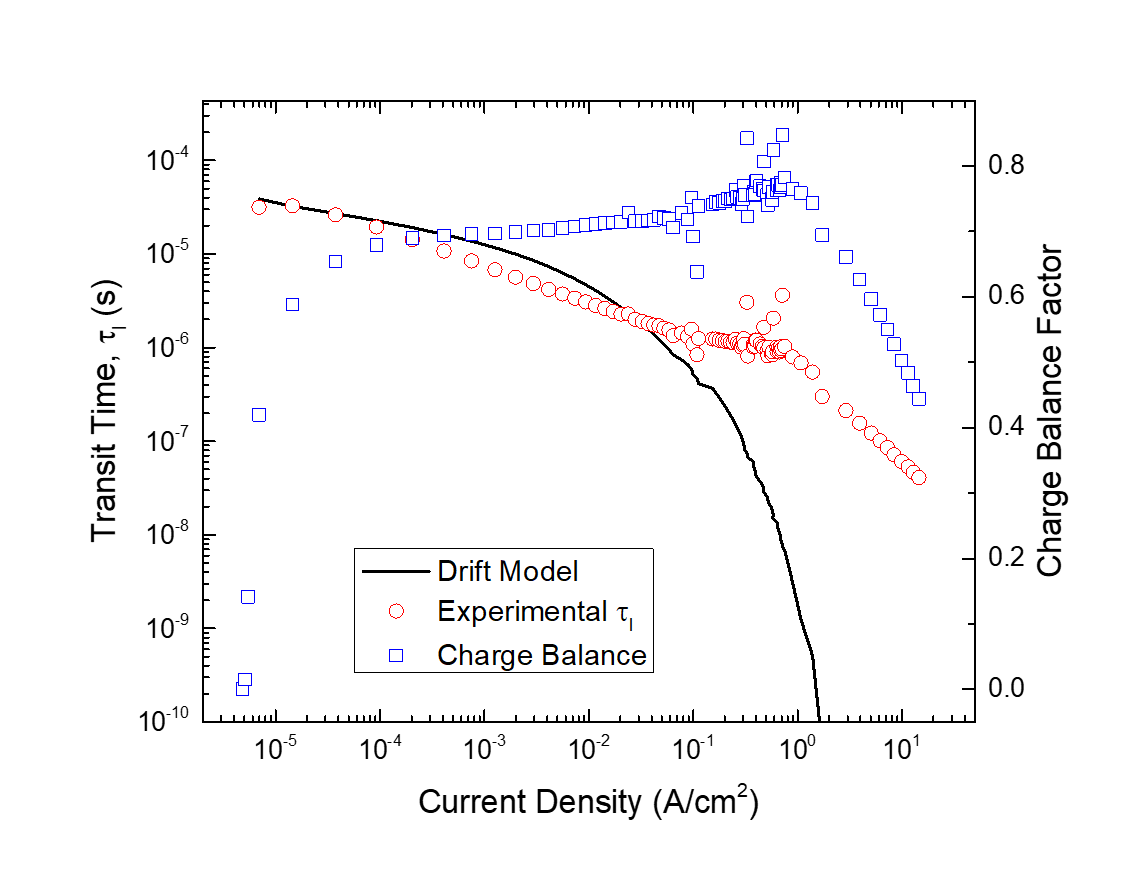
\includegraphics[width=0.48\textwidth]{unified/chargeBalance}
\caption{Transit time extracted from $\eta_{EQE}$ measurements are shown as the red circles. Predictions using the drift model are calculated using Eqn. \ref{eqn:drift}. The drift model assumes a uniform electric field. Good agreement between the experimental transit time and the drift model is found for a field distributed over 20 nm. The charge balance factor is shown as a function of current density in blue squares.}
\label{fig:chargeBalance}
\end{wrapfigure}
\subsection{Drift Model}

\begin{equation}
\tau_l=\frac{w}{E\mu(E)}
\label{eqn:drift}
\end{equation}


\section{Understanding Assumptions of Polaron Model}
\subsection{Carrier Injection}

\begin{equation}
\frac{dn_h}{dt}=-k_Fn_en_h-\frac{n_h}{\tau_{lh}}+\frac{J_h}{ew}
\label{eqn:hole_rate}
\end{equation}

\begin{equation}
\frac{dn_e}{dt}=-k_Fn_en_h-\frac{n_e}{\tau_{le}}+\frac{J_e}{ew}
\label{eqn:electron_rate}
\end{equation}

\begin{equation}
J_1\rightarrow J_h = J_2 \rightarrow J_e
\label{eqn:current_no_leakage}
\end{equation}

\begin{equation}
\frac{J_e}{ew}+\frac{J_h}{ew}=\frac{J_1+J_2}{ew}=\frac{2J}{ew}
\label{eqn:injected_polarons_no_leakage}
\end{equation}

\begin{equation}
J_1=J_h
\label{eqn:current_holes_leakage}
\end{equation}

\begin{equation}
J_2=J_e+J_l
\label{eqn:current_electrons_leakage}
\end{equation}

\begin{equation}
J=J_h=J_e+J_l
\label{eqn:current_continuity_leakage}
\end{equation}

\begin{equation}
G_{pol}-\frac{J_l}{ew}=\frac{2J-J_l}{ew}
\label{polaron_generation}
\end{equation}

\subsection{Charge Imbalance}

\begin{equation}
\alpha=\frac{n_h}{n_e+n_h}
\label{eqn:charge_ratio}
\end{equation}

\begin{equation}
\left[\frac{dn_{pol}}{dt}\right]_{formation}=-2k_Fn_{pol}^2\alpha(1-\alpha)
\label{eqn:exciton_formation_charge_ratio}
\end{equation}



\begin{wrapfigure}{r}{0.5\textwidth}
\centering
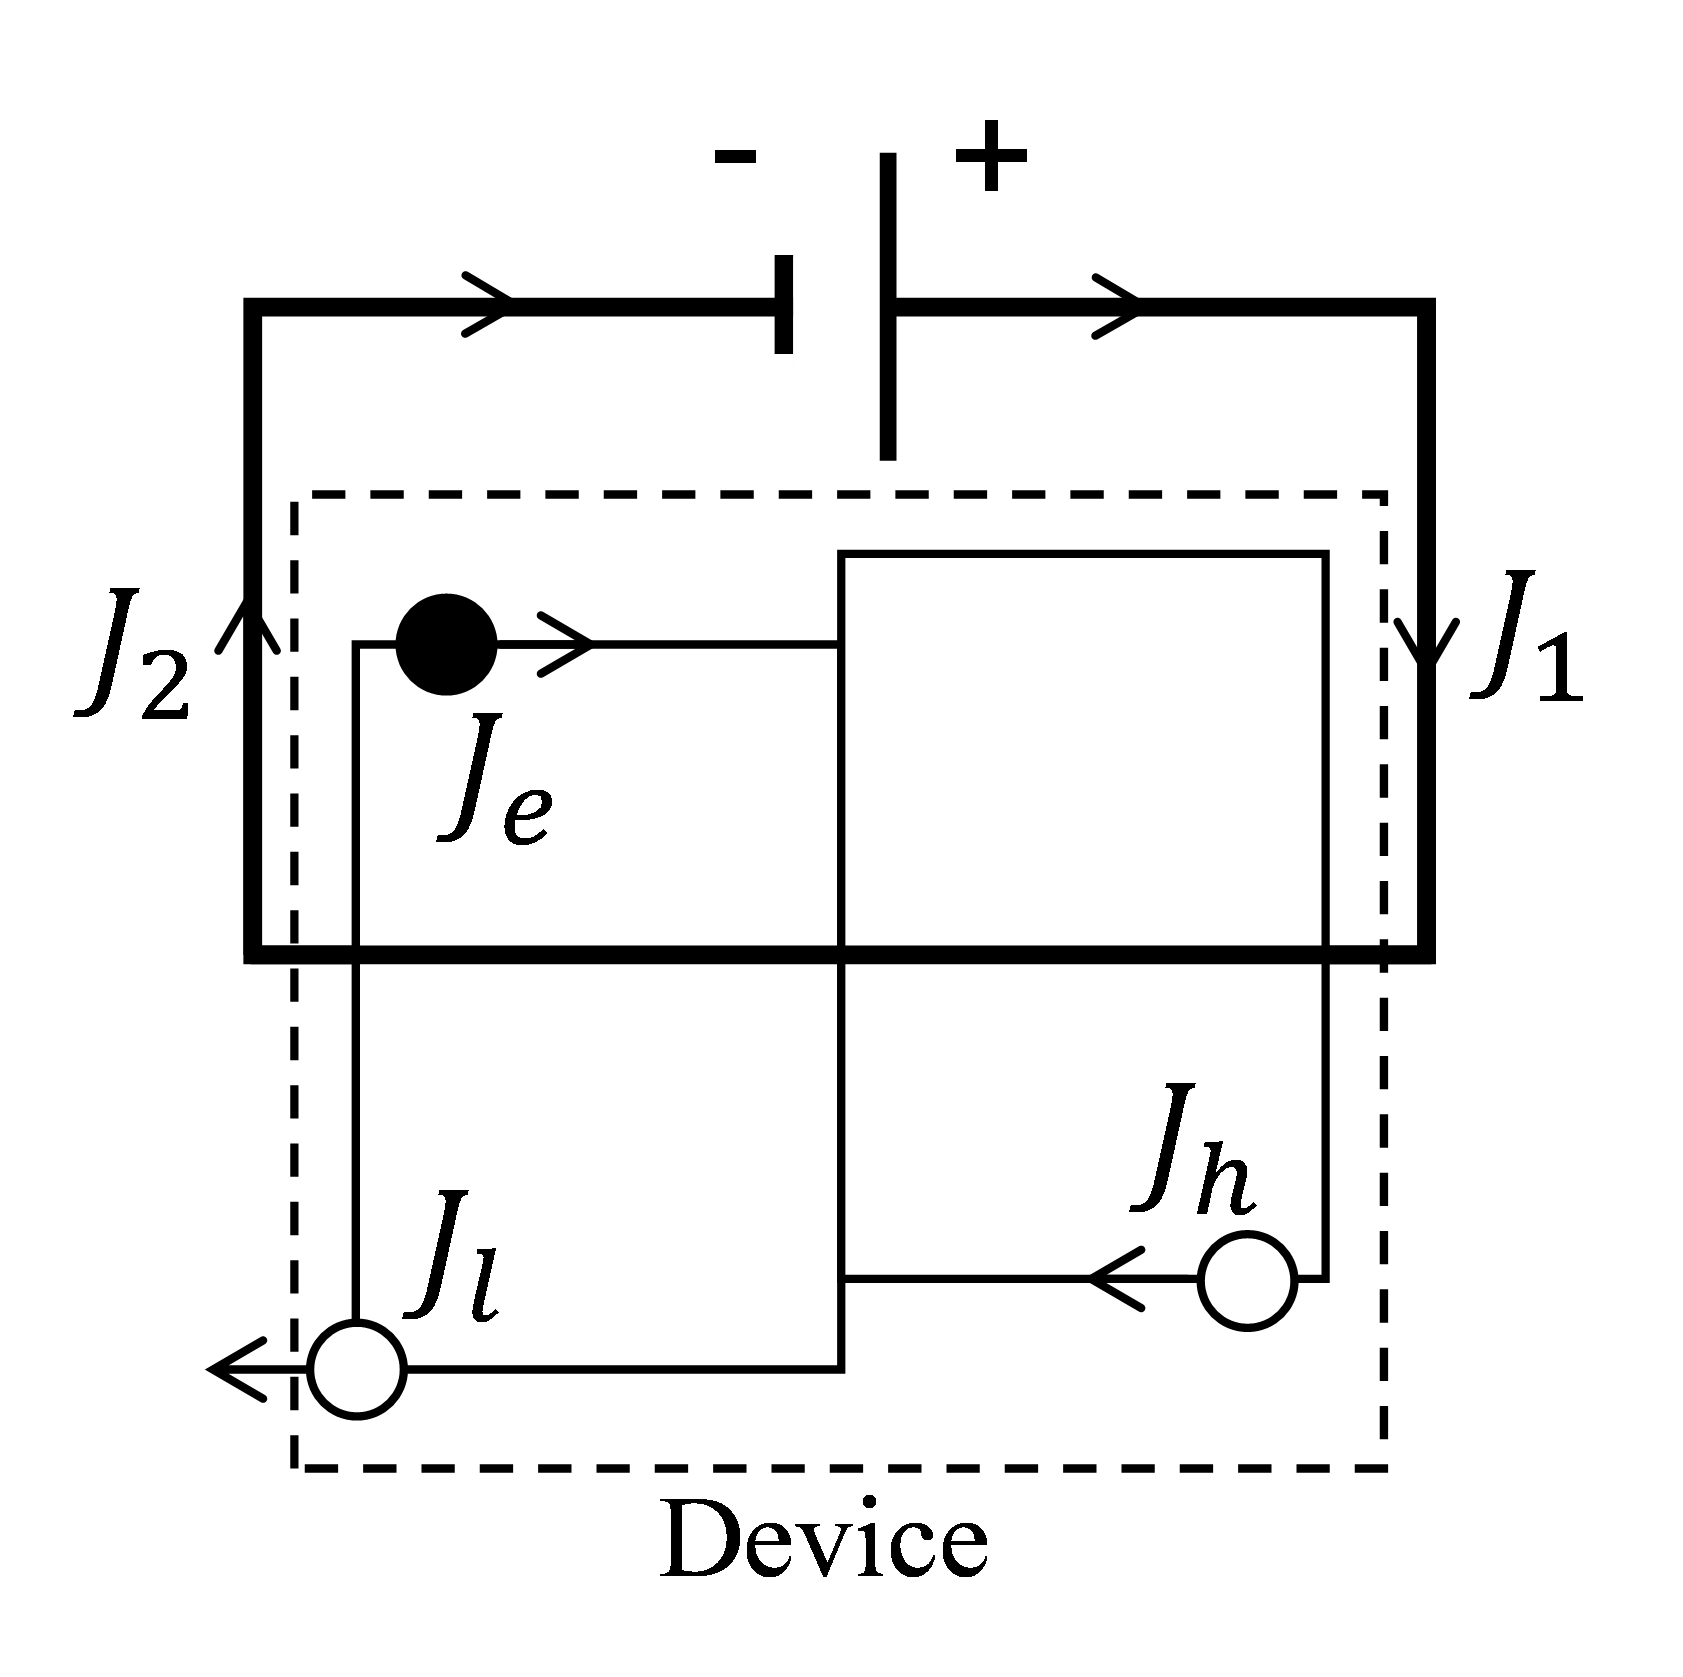
\includegraphics[scale=.1]{unified/currentDiagram}
\caption{Current density formalism within the circuit. and are the currents measured on either side of the device. and are the electron and hole currents within the device and is the unbalanced current, assumed to be only holes, that leaks out of the opposing contact.}
\label{fig:currentDiagram}
\end{wrapfigure}

\begin{wrapfigure}{r}{0.5\textwidth}
\centering
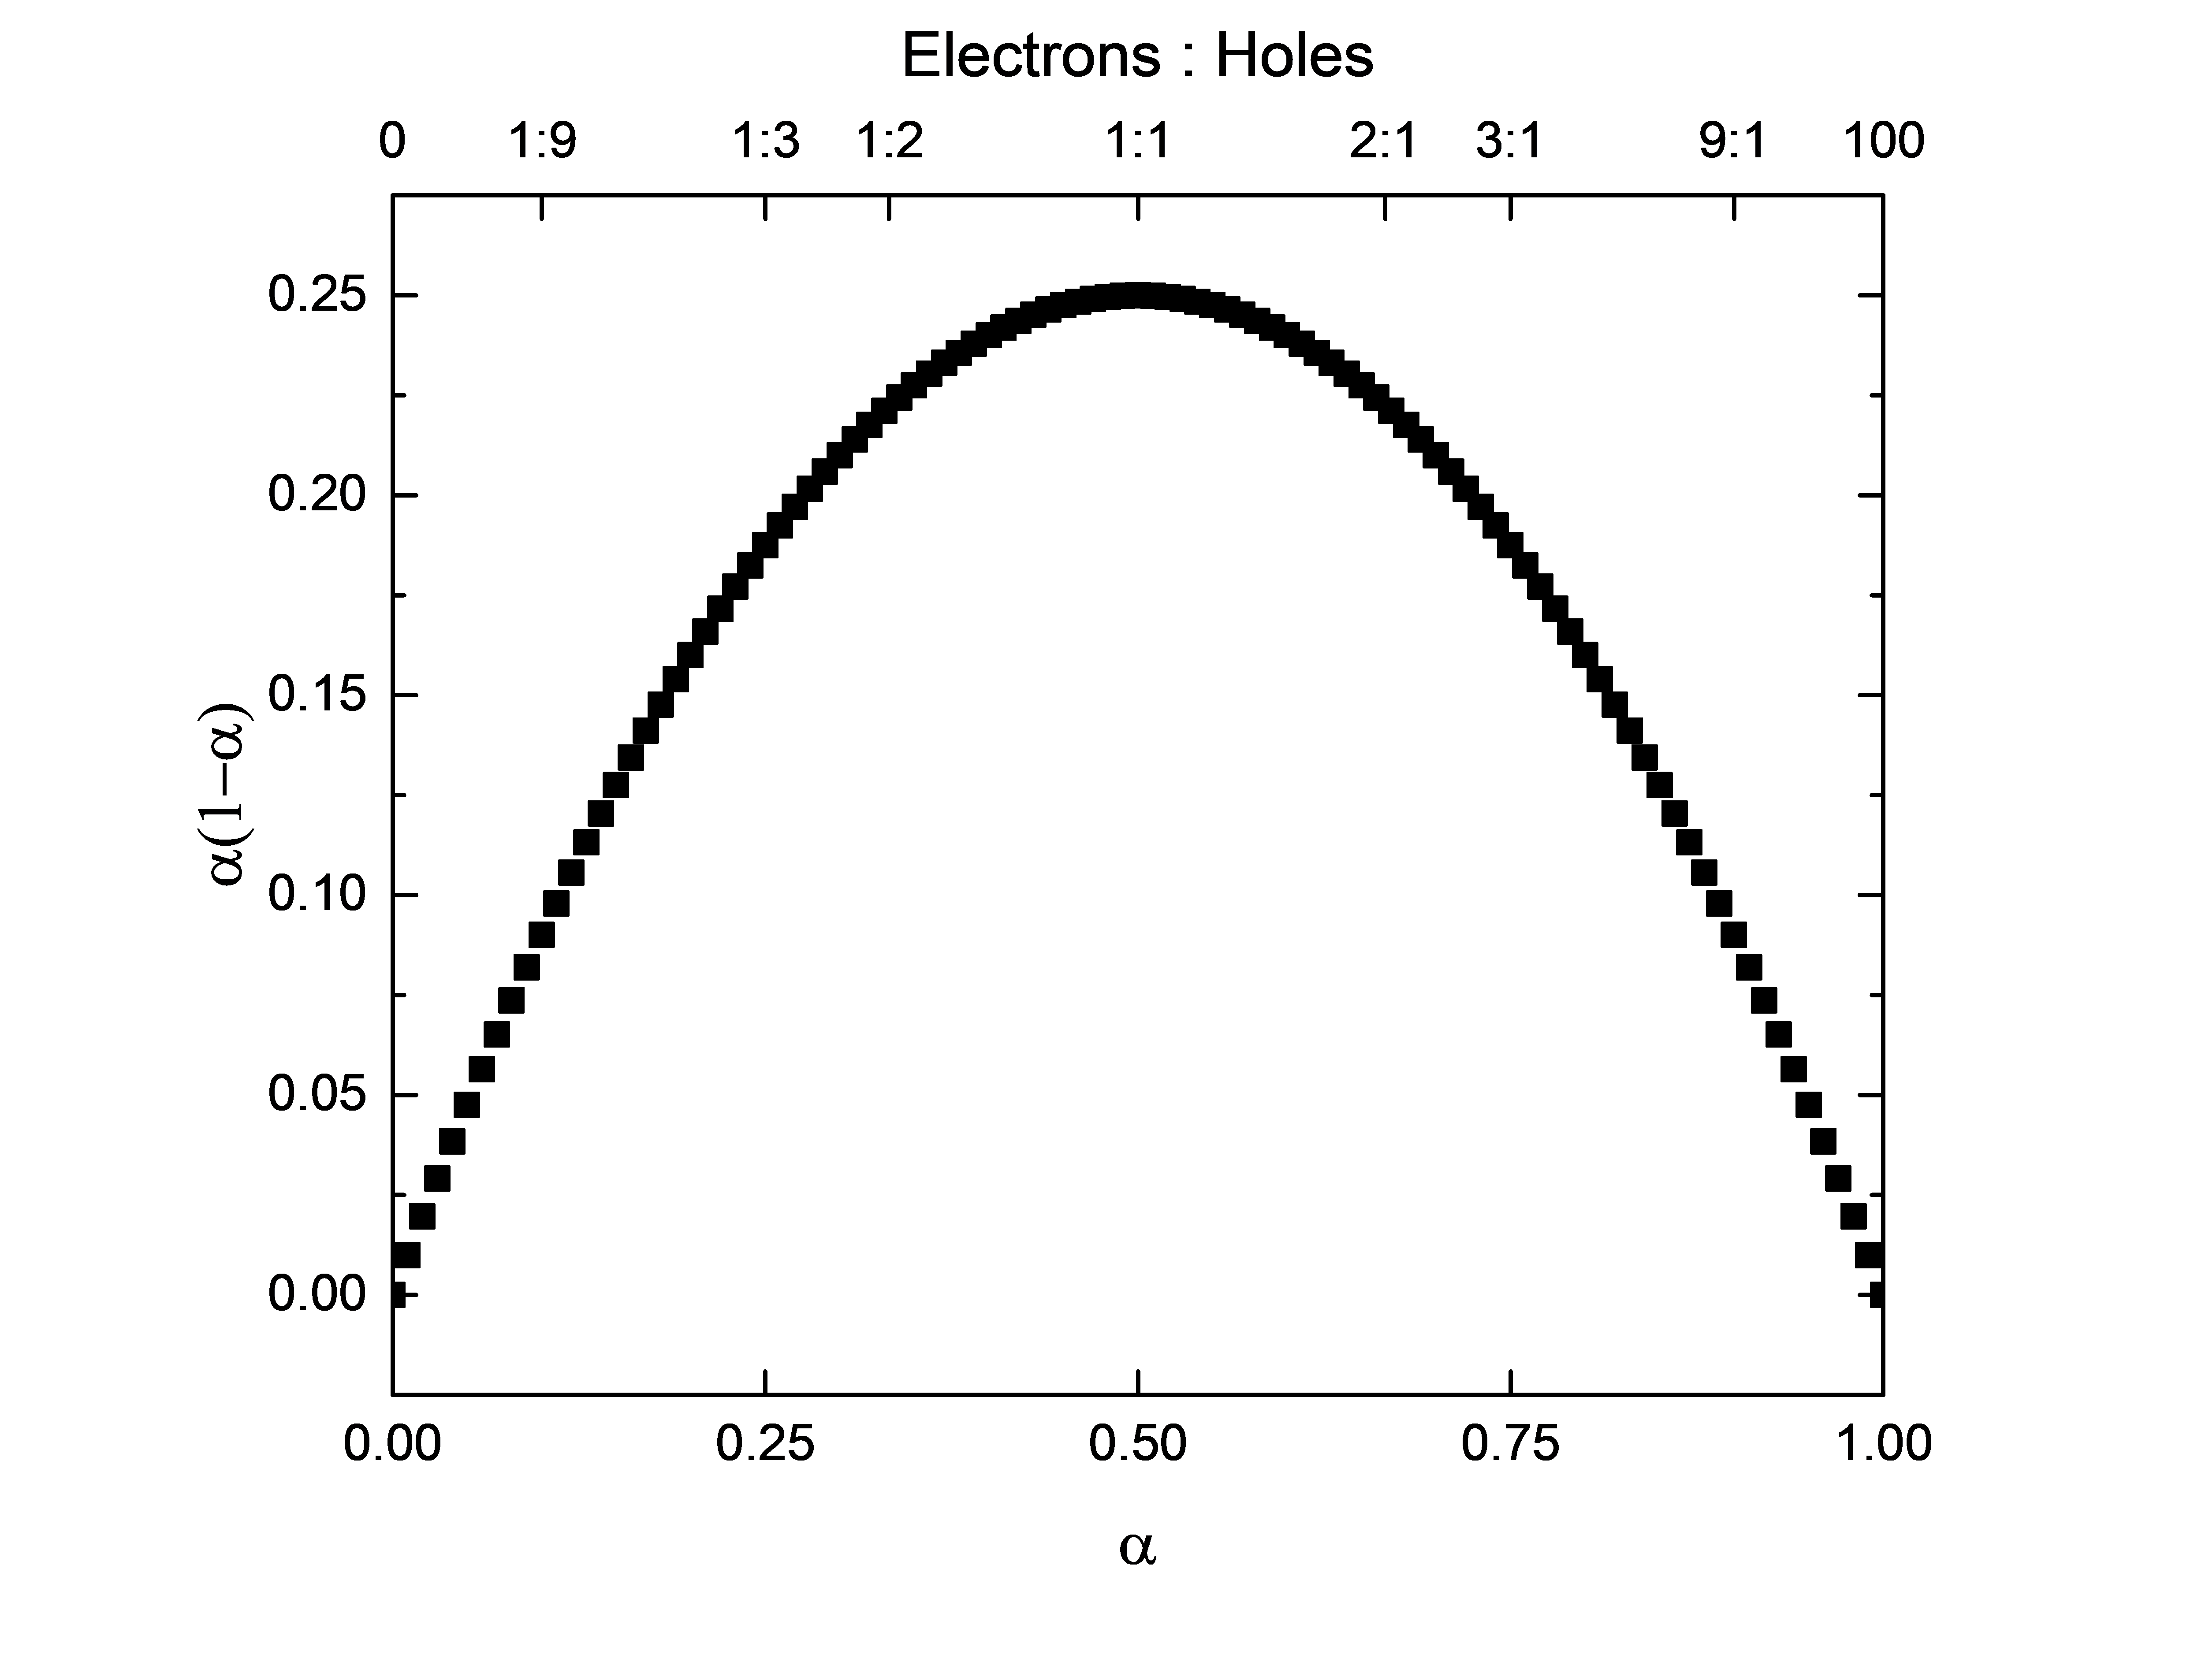
\includegraphics[scale=.1]{unified/EHratio}
\caption{The quantity $\alpha(1-\alpha)$ is plotted as a function of the polaron composition, $\alpha$ and the electron to hole ratio.}
\label{fig:EHratio}
\end{wrapfigure}

\ifcsdef{mainfile}{}{\bibliography{../thesis}}
\end{document}

